\documentclass[12pt]{article}
\usepackage[dvipsnames, table, xcdraw]{xcolor}

\usepackage[margin=1in]{geometry} 
\usepackage{amsmath,amsthm,amssymb,color}
\usepackage{graphicx}
\usepackage{mathtools}
\usepackage{mathdots}
\usepackage{centernot}
\usepackage{algorithm}
\usepackage[noend]{algpseudocode}
\usepackage{csquotes}
\usepackage{enumerate}
\usepackage{tikz}
\usetikzlibrary{calc}
\usepackage{bbm}
\usetikzlibrary{arrows, shapes}
\usetikzlibrary{patterns}
\usepackage{relsize}
\usetikzlibrary{decorations.pathreplacing}
\allowdisplaybreaks


\begin{document}

\begin{figure}[htbp] %  figure placement: here, top, bottom, or page
   \centering
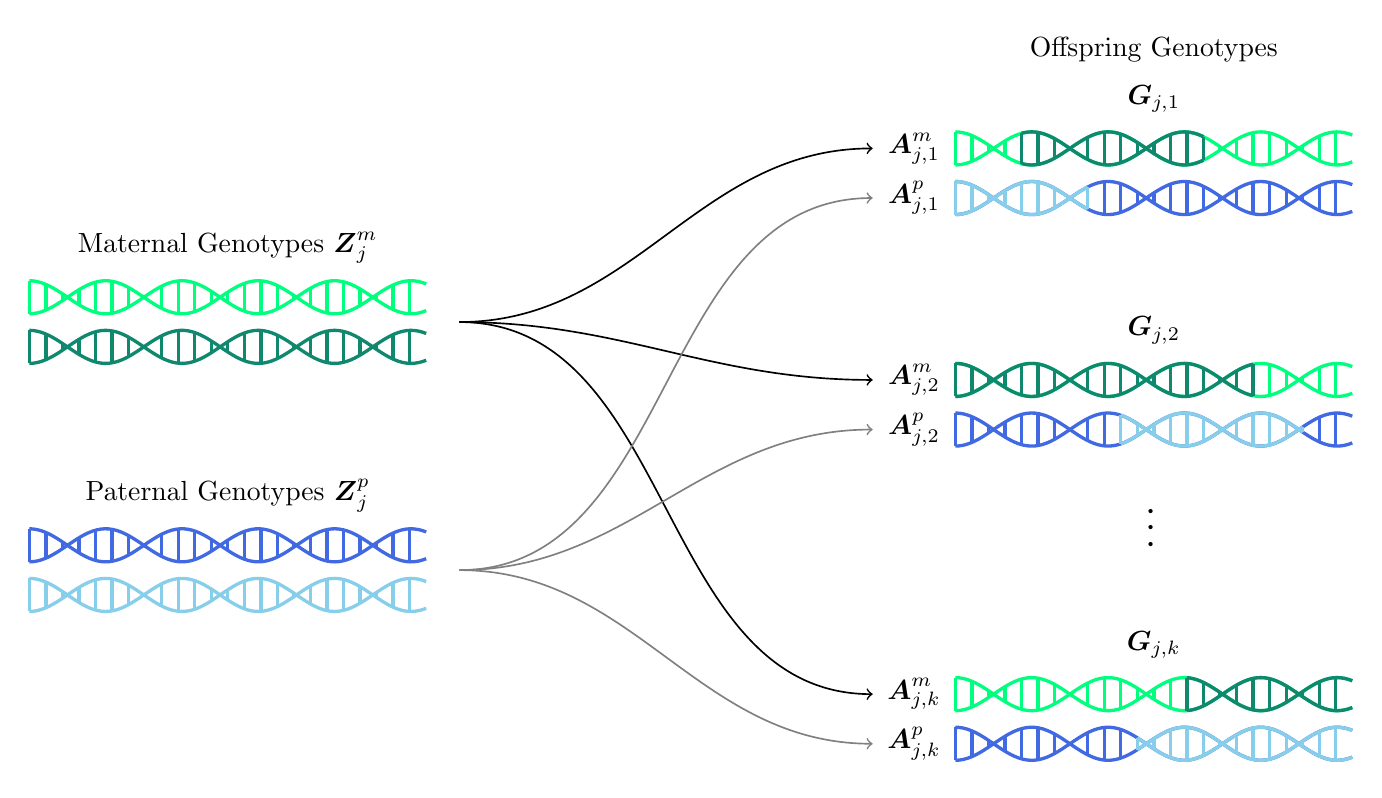
\begin{tikzpicture}[scale=3]
    \def\zmmx{-28}; % maternal genotype x coordinate
    \def\zmmy{9}; % maternal genotype y coordinate
    \def\zmpx{-28}; % maternal genotype x coordinate
    \def\zmpy{6}; % maternal genotype y coordinate
    
    \def\zpmx{-28}; % paternal genotype x coordinate
    \def\zpmy{-6}; % paternal genotype y coordinate
    \def\zppx{-28}; % paternal genotype x coordinate
    \def\zppy{-9}; % paternal genotype y coordinate
    
    \def\amax{28}; % child a maternal allele x coordinate
    \def\amay{18}; % child a maternal allele y coordinate
    \def\apax{28}; % child a patenral allele x coordinate
    \def\apay{15}; % child a paternal allele y coordinate
    
    \def\ambx{28}; % child b maternal allele x coordinate
    \def\amby{4}; % child b maternal allele y coordinate
    \def\apbx{28}; % child b patenral allele x coordinate
    \def\apby{1}; % child b paternal allele y coordinate
    
    \def\amcx{28}; % child c maternal allele x coordinate
    \def\amcy{-15}; % child c maternal allele y coordinate
    \def\apcx{28}; % child c patenral allele x coordinate
    \def\apcy{-18}; % child c paternal allele y coordinate
    
    
    \def\mpcol{PineGreen}; % maternal genotypes color
	\def\mmcol{SpringGreen};
	\def\ppcol{SkyBlue}; % paternal genotypes color
	\def\pmcol{RoyalBlue};
	
	
	\begin{scope}[scale=.07, domain=0:24, samples=101]
	    
	    % background color %%%%%%%%%%%%%%%%%%%%%%%%%%%%%%%%%%%%%%%%%%%%%%%%%%%%%%%%%%%%%%%%%%%%%%%%%%%
        \foreach \x in {0,1, ...,23}{
          % maternal genotypes 
          \draw[very thick, \mmcol] (\x + \zmmx,{-cos(\x*39) + \zmmy}) -- (\x + \zmmx,{cos(\x*39) + \zmmy});
          \draw[very thick, \mpcol] (\x + \zmpx,{-cos(\x*39) + \zmpy}) -- (\x + \zmpx,{cos(\x*39) + \zmpy});
          % paternal genotypes
          \draw[very thick, \pmcol] (\x + \zpmx,{-cos(\x*39) + \zpmy}) -- (\x + \zpmx,{cos(\x*39) + \zpmy});
          \draw[very thick, \ppcol] (\x + \zppx,{-cos(\x*39) + \zppy}) -- (\x + \zppx,{cos(\x*39) + \zppy});
        }
        % maternal genotypes %%%%%%%%%%%%%%%%%%%%%%%%%%%%%%%%%%%%%%%%%%%%%%%%%%%%%%%%%%%%%%%%%%%%%%%%%
        \draw[\mmcol, very thick] plot (\x + \zmmx, {cos(\x*39) + \zmmy });
        \draw[\mmcol, very thick] plot (\x + \zmmx, {-cos(\x*39) + \zmmy});
        \draw[\mpcol, very thick] plot (\x + \zmpx, {cos(\x*39) + \zmpy });
        \draw[\mpcol, very thick] plot (\x + \zmpx, {-cos(\x*39) + \zmpy});
        % paternal genotypes %%%%%%%%%%%%%%%%%%%%%%%%%%%%%%%%%%%%%%%%%%%%%%%%%%%%%%%%%%%%%%%%%%%%%%%%%
        \draw[\pmcol, very thick] plot (\x + \zpmx, {cos(\x*39) + \zpmy });
        \draw[\pmcol, very thick] plot (\x + \zpmx, {-cos(\x*39) + \zpmy});
        \draw[\ppcol, very thick] plot (\x + \zppx, {cos(\x*39) + \zppy });
        \draw[\ppcol, very thick] plot (\x + \zppx, {-cos(\x*39) + \zppy});
        % offspring a genotypes %%%%%%%%%%%%%%%%%%%%%%%%%%%%%%%%%%%%%%%%%%%%%%%%%%%%%%%%%%%%%%%%%%%%%%
        \draw[\mmcol, domain=0:24, very thick] plot (\x + \amax, {cos(\x*39) + \amay });
        \draw[\mmcol, domain=0:24, very thick] plot (\x + \amax, {-cos(\x*39) + \amay });
        \draw[\mpcol, domain=4:15, very thick] plot (\x + \amax, {cos(\x*39) + \amay });
        \draw[\mpcol, domain=4:15, very thick] plot (\x + \amax, {-cos(\x*39) + \amay });
        \draw[\pmcol, domain=0:24, very thick] plot (\x + \apax, {cos(\x*39) + \apay });
        \draw[\pmcol, domain=0:24, very thick] plot (\x + \apax, {-cos(\x*39) + \apay });
        \draw[\ppcol, domain=0:8, very thick] plot (\x + \apax, {cos(\x*39) + \apay });
        \draw[\ppcol, domain=0:8, very thick] plot (\x + \apax, {-cos(\x*39) + \apay });
        \foreach \x in {0,1, ...,23}{
          \draw[very thick, \mmcol] (\x + \amax,{-cos(\x*39) + \amay}) -- (\x + \amax,{cos(\x*39) + \amay});
          \draw[very thick, \pmcol] (\x + \apax,{-cos(\x*39) + \apay}) -- (\x + \apax,{cos(\x*39) + \apay});
        }
        \foreach \x in {4,5, ...,15}{
          \draw[very thick, \mpcol] (\x + \amax,{-cos(\x*39) + \amay}) -- (\x + \amax,{cos(\x*39) + \amay});
        }
        \foreach \x in {0,1, ...,8}{
          \draw[very thick, \ppcol] (\x + \apax,{-cos(\x*39) + \apay}) -- (\x + \apax,{cos(\x*39) + \apay});
        }
        % offspring b genotypes %%%%%%%%%%%%%%%%%%%%%%%%%%%%%%%%%%%%%%%%%%%%%%%%%%%%%%%%%%%%%%%%%%%%%%
        \draw[\mmcol, domain=0:24, very thick] plot (\x + \ambx, {cos(\x*39) + \amby });
        \draw[\mmcol, domain=0:24, very thick] plot (\x + \ambx, {-cos(\x*39) + \amby });
        \draw[\mpcol, domain=0:18, very thick] plot (\x + \ambx, {cos(\x*39) + \amby });
        \draw[\mpcol, domain=0:18, very thick] plot (\x + \ambx, {-cos(\x*39) + \amby });
        \draw[\pmcol, domain=0:24, very thick] plot (\x + \apbx, {cos(\x*39) + \apby });
        \draw[\pmcol, domain=0:24, very thick] plot (\x + \apbx, {-cos(\x*39) + \apby });
        \draw[\ppcol, domain=10:21, very thick] plot (\x + \apbx, {cos(\x*39) + \apby });
        \draw[\ppcol, domain=10:21, very thick] plot (\x + \apbx, {-cos(\x*39) + \apby });
        \foreach \x in {0,1, ...,23}{
          \draw[very thick, \mmcol] (\x + \ambx,{-cos(\x*39) + \amby}) -- (\x + \amax,{cos(\x*39) + \amby});
          \draw[very thick, \pmcol] (\x + \apbx,{-cos(\x*39) + \apby}) -- (\x + \apax,{cos(\x*39) + \apby});
        }
        \foreach \x in {0,1, ...,18}{
          \draw[very thick, \mpcol] (\x + \ambx,{-cos(\x*39) + \amby}) -- (\x + \amax,{cos(\x*39) + \amby});
        }
        \foreach \x in {10,11, ...,21}{
          \draw[very thick, \ppcol] (\x + \apbx,{-cos(\x*39) + \apby}) -- (\x + \apax,{cos(\x*39) + \apby});
        }
        % offspring c genotypes %%%%%%%%%%%%%%%%%%%%%%%%%%%%%%%%%%%%%%%%%%%%%%%%%%%%%%%%%%%%%%%%%%%%%%
        \draw[\mmcol, domain=0:24, very thick] plot (\x + \amcx, {cos(\x*39) + \amcy });
        \draw[\mmcol, domain=0:24, very thick] plot (\x + \amcx, {-cos(\x*39) + \amcy });
        \draw[\mpcol, domain=14:24, very thick] plot (\x + \amcx, {cos(\x*39) + \amcy });
        \draw[\mpcol, domain=14:24, very thick] plot (\x + \amcx, {-cos(\x*39) + \amcy });
        \draw[\pmcol, domain=0:24, very thick] plot (\x + \apcx, {cos(\x*39) + \apcy });
        \draw[\pmcol, domain=0:24, very thick] plot (\x + \apcx, {-cos(\x*39) + \apcy });
        \draw[\ppcol, domain=11:24, very thick] plot (\x + \apcx, {cos(\x*39) + \apcy });
        \draw[\ppcol, domain=11:24, very thick] plot (\x + \apcx, {-cos(\x*39) + \apcy });
        \foreach \x in {0,1, ...,23}{
          \draw[very thick, \mmcol] (\x + \amcx,{-cos(\x*39) + \amcy}) -- (\x + \amax,{cos(\x*39) + \amcy});
          \draw[very thick, \pmcol] (\x + \apcx,{-cos(\x*39) + \apcy}) -- (\x + \apax,{cos(\x*39) + \apcy});
        }
        \foreach \x in {14,15, ...,23}{
          \draw[very thick, \mpcol] (\x + \amcx,{-cos(\x*39) + \amcy}) -- (\x + \amax,{cos(\x*39) + \amcy});
        }
        \foreach \x in {11,12, ...,23}{
          \draw[very thick, \ppcol] (\x + \apcx,{-cos(\x*39) + \apcy}) -- (\x + \apax,{cos(\x*39) + \apcy});
        }        
        % annotations %%%%%%%%%%%%%%%%%%%%%%%%%%%%%%%%%%%%%%%%%%%%%%%%%%%%%%%%%%%%%%%%%%%%%%%%%%%%%%%%%   
        \node at (\zmmx + 12, \zmmy + 3) {Maternal Genotypes $\boldsymbol{Z}^m_j$};
        \node at (\zpmx + 12, \zpmy + 3) {Paternal Genotypes $\boldsymbol{Z}^p_j$};
        \node at (\amax + 12, \amay + 6) {Offspring Genotypes};
        \node at (\amax + 12, \amay + 3) {$\boldsymbol{G}_{j,1}$};
        \node at (\amax-2.5, \amay) {$\boldsymbol{A}^m_{j,1}$};
        \node at (\apax-2.5, \apay) {$\boldsymbol{A}^p_{j,1}$};
        \node at (\ambx + 12, \amby + 3) {$\boldsymbol{G}_{j,2}$};
        \node at (\ambx-2.5, \amby) {$\boldsymbol{A}^m_{j,2}$};
        \node at (\apbx-2.5, \apby) {$\boldsymbol{A}^p_{j,2}$};
        \node at (\apbx + 11.8, \apby - 5) {\Large$\cdot$};
        \node at (\apbx + 11.8, \apby - 6) {\Large$\cdot$};
        \node at (\apbx + 11.8, \apby - 7) {\Large$\cdot$};
        \node at (\amcx + 12, \amcy + 3) {$\boldsymbol{G}_{j,k}$};
        \node at (\amcx-2.5, \amcy) {$\boldsymbol{A}^m_{j,k}$};
        \node at (\apcx-2.5, \apcy) {$\boldsymbol{A}^p_{j,k}$};
        % arrows %%%%%%%%%%%%%%%%%%%%%%%%%%%%%%%%%%%%%%%%%%%%%%%%%%%%%%%%%%%%%%%%%%%%%%%%%%%%%%%%%%%%%%
        \draw[->, line width = 0.6, color = black] (\zmmx+26, \zmmy/2+\zmpy/2) to [out=0,in=180] (\amax-5, \amay);
        \draw[->, line width = 0.6, color = black] (\zmmx+26, \zmmy/2+\zmpy/2) to [out=0,in=180] (\ambx-5, \amby);
        \draw[->, line width = 0.6, color = black] (\zmmx+26, \zmmy/2+\zmpy/2) to [out=0,in=180] (\amcx-5, \amcy);
        \draw[->, line width = 0.6, color = gray] (\zpmx+26, \zpmy/2+\zppy/2) to [out=0,in=180] (\apax-5, \apay);
        \draw[->, line width = 0.6, color = gray] (\zpmx+26, \zpmy/2+\zppy/2) to [out=0,in=180] (\apbx-5, \apby);
        \draw[->, line width = 0.6, color = gray] (\zpmx+26, \zpmy/2+\zppy/2) to [out=0,in=180] (\apcx-5, \apcy);
        
        % straight arrows %%%%%%%%%%%%%%%%%%%%%%%%%%%%%%%%%%%%%%%%%%%%%%%%%%%%%%%%%%%%%%%%%%%%%%%%%%%%%
        % \draw[->, line width = 0.6, color = black] (\zmmx+26, \zmmy/2+\zmpy/2) to (\amax-5, \amay);
        % \draw[->, line width = 0.6, color = black] (\zmmx+26, \zmmy/2+\zmpy/2) to (\ambx-5, \amby);
        % \draw[->, line width = 0.6, color = black] (\zmmx+26, \zmmy/2+\zmpy/2) to (\amcx-5, \amcy);
        % \draw[->, line width = 0.6, color = gray] (\zpmx+26, \zpmy/2+\zppy/2) to (\apax-5, \apay);
        % \draw[->, line width = 0.6, color = gray] (\zpmx+26, \zpmy/2+\zppy/2) to (\apbx-5, \apby);
        % \draw[->, line width = 0.6, color = gray] (\zpmx+26, \zpmy/2+\zppy/2) to (\apcx-5, \apcy);
        
        
    \end{scope}
 	

	
	
\end{tikzpicture}
\end{figure}


\end{document}